%%%%%%%%%%%%%%%%%%%%%%%%%%%%%%%%%%%%%%%%%%%%%%%%%%%%%%%%%%%%%%%%%%%%%%%%%%%%%%%
%                       CARGA DE LA CLASE DE DOCUMENTO                        %
%                                                                             %
% Las opciones admisibles son:                                                %
%      12pt / 11pt            (tamaño del cuerpo de letra; no usar 10pt)      %
%                                                                             %
% catalan/spanish/english     (idioma principal del trabajo)                  %
%                                                                             % 
% french/italian/german...    (si necesitáis usar otro idioma adicional)      %
%                                                                             %
% listoffigures               (El documento incluye un Índice de figuras)     %
% listoftables                (El documento incluye un Índice de tablas)      %
% listofquadres               (El documento incluye un Índice de cuadros)     %
% listofalgorithms            (El documento incluye un Índice de algoritmos)  %
%                                                                             %
%%%%%%%%%%%%%%%%%%%%%%%%%%%%%%%%%%%%%%%%%%%%%%%%%%%%%%%%%%%%%%%%%%%%%%%%%%%%%%%

\documentclass[11pt,spanish,listoffigures,listoftables]{tfgetsinf}

%%%%%%%%%%%%%%%%%%%%%%%%%%%%%%%%%%%%%%%%%%%%%%%%%%%%%%%%%%%%%%%%%%%%%%%%%%%%%%%
%                     CODIFICACIÓN DEL ARCHIVO FUENTE                         %
%                                                                             %
%    Windows suele usar 'ansinew'                                             %
%    en Linux es posible que sea 'latin1' o 'latin9'                          %
%    Pero lo más recomendable es usar utf8 (unicode 8)                        %
%                                          (si vuestro editor lo permite)     % 
%%%%%%%%%%%%%%%%%%%%%%%%%%%%%%%%%%%%%%%%%%%%%%%%%%%%%%%%%%%%%%%%%%%%%%%%%%%%%%%

\usepackage[utf8]{inputenc} 


%%%%%%%%%%%%%%%%%%%%%%%%%%%%%%%%%%%%%%%%%%%%%%%%%%%%%%%%%%%%%%%%%%%%%%%%%%%%%%%
%                       OTROS PAQUETES Y DEFINICIONES                         %
%                                                                             %
%%%%%%%%%%%%%%%%%%%%%%%%%%%%%%%%%%%%%%%%%%%%%%%%%%%%%%%%%%%%%%%%%%%%%%%%%%%%%%%

\usepackage{glossaries}
\usepackage{textcomp}
\usepackage{booktabs}
\usepackage{float}
\usepackage{enumitem}
\usepackage{graphicx}
\usepackage{subcaption}
\usepackage{tabularx}
\usepackage{pgfplots}
\usepackage{amsmath}  % For \xrightarrow
\usepackage{tikz-cd}  % For the diagram arrow with text inside
\pgfplotsset{compat=1.18}
\usepgfplotslibrary{groupplots}
\usetikzlibrary{calc}
\usetikzlibrary{babel}  % Compatibility with Spanish babel active "
% Listings para código
\usepackage{listings}
\lstset{
  basicstyle=\ttfamily\small,
  frame=single,
  breaklines=true,
  postbreak=\mbox{\textcolor{gray}{$\hookrightarrow$}\space},
  columns=fullflexible,
  keepspaces=true,
  numbers=none
}

% Bibliografía
\usepackage[backend=biber,style=numeric,sorting=none]{biblatex}
\addbibresource{bibliografia.bib}

% Hyperref siempre al final
\usepackage{hyperref}
\hypersetup{
  colorlinks=true,
  linkcolor=black,
  urlcolor=cyan,
  citecolor=black
}
%%%%%%%%%%%%%%%%%%%%%%%%%%%%%%%%%%%%%%%%%%%%%%%%%%%%%%%%%%%%%%%%%%%%%%%%%%%%%%%
%                          DATOS DEL TRABAJO                                  %
%                                                                             %
% título alumno, titor y curso académico                                      %
%%%%%%%%%%%%%%%%%%%%%%%%%%%%%%%%%%%%%%%%%%%%%%%%%%%%%%%%%%%%%%%%%%%%%%%%%%%%%%%

\title{Biometría: Filtros, Curvas ROC y Detector facial Viola Jones}
\author{Gómez Corral, Miquel}
% \tutor{No}
% \curs{MUIARFID}

%%%%%%%%%%%%%%%%%%%%%%%%%%%%%%%%%%%%%%%%%%%%%%%%%%%%%%%%%%%%%%%%%%%%%%%%%%%%%%%
%                     PARAULES CLAU/PALABRAS CLAVE/KEY WORDS                  %
%                                                                             %
% Independentment de la llengua del treball, s'hi han d'incloure              %
% les paraules clau i el resum en els tres idiomes                            %
%%%%%%%%%%%%%%%%%%%%%%%%%%%%%%%%%%%%%%%%%%%%%%%%%%%%%%%%%%%%%%%%%%%%%%%%%%%%%%%

\keywords{
    Machine Learning; Detección facial; Curva ROC; Viola Jones; AdaBoost;
} % Paraules clau 
{
    Machine Learning; Face Detection; ROC Curve; Viola Jones; AdaBoost;
} % Palabras clave
{
    Machine Learning; Face Detection; ROC Curve; Viola Jones; AdaBoost;
} % Key words


%%%%%%%%%%%%%%%%%%%%%%%%%%%%%%%%%%%%%%%%%%%%%%%%%%%%%%%%%%%%%%%%%%%%%%%%%%%%%%%
%                                                                             %
%                              INICI DEL DOCUMENT                             %
%                                                                             %
%%%%%%%%%%%%%%%%%%%%%%%%%%%%%%%%%%%%%%%%%%%%%%%%%%%%%%%%%%%%%%%%%%%%%%%%%%%%%%%

\begin{document} 


%%%%%%%%%%%%%%%%%%%%%%%%%%%%%%%%%%%%%%%%%%%%%%%%%%%%%%%%%%%%%%%%%%%%%%%%%%%%%%%
%              RESUMENES DEL TFG EN VALENCIA, CASTELLA I ANGLES               %
%%%%%%%%%%%%%%%%%%%%%%%%%%%%%%%%%%%%%%%%%%%%%%%%%%%%%%%%%%%%%%%%%%%%%%%%%%%%%%%


% \begin{abstract}[spanish]

% \end{abstract}

%%%%%%%%%%%%%%%%%%%%%%%%%%%%%%%%%%%%%%%%%%%%%%%%%%%%%%%%%%%%%%%%%%%%%%%%%%%%%%%
%                                                                             %
%                              CONTENIDO DEL TREBAJO                          %
%                                                                             %
%%%%%%%%%%%%%%%%%%%%%%%%%%%%%%%%%%%%%%%%%%%%%%%%%%%%%%%%%%%%%%%%%%%%%%%%%%%%%%%

%%%%%%%%%%%%%%%%%%%%%%%%%%%%%%%%%%%%%%%%%%%%%%%%%%%%%%%%%%%%%%%%%%%%%%%%%%%%%%%
% ÍNDICE                                     %
%%%%%%%%%%%%%%%%%%%%%%%%%%%%%%%%%%%%%%%%%%%%%%%%%%%%%%%%%%%%%%%%%%%%%%%%%%%%%%%
% \clearpage
% \tableofcontents
% \listoffigures
% \listoftables


\mainmatter

\chapter{Introducción}

% I want you to write down these sections. use as base the enumerate I added above, and include some implementation details
% For that, I want you to explore the repository


% also, include this:
% -  The dataset from which I get the non face samples is from fiftyone: "open-images-v7". Since there are no faces, (almost all the time), we predist with the current stage, and all the crops returned as images are FP. The dataset HAS many images with faces, but we filter by some tags that nearly all have imagas that do not include faces, These labels are generated with 'app/scripts/generate_labels.py'
% - for the features we just loop over all the positions and sizes of the verticall and horizontal filters. We just care about one way, not both (like black-white and not the other way) bc the Ada boost manages sign of the input features
% - we precompute once all the faces features, but the hard mining ones are taken on the fly bc at each stage the non-faces crops change
% - All the haar filters are computed with the intergral image techinique
% - Claude LLM provided an implementation of the Adaboost algorith that maches the features of sklearn but, just uses stumps and is faster when looking for each stump spilt across all features: it does it on paralel. 
% - for each stage we train the adaboost to select best features, then, we prune the forest by cheking at which stages we get (adjusting the threshold) high TF and 50% FN to reduce stage size
% - To generate the balanced dataset, we reuse the crops that passed the last stage + generate the remaining (up to the number of faces for balanced dataset) by predictig with the clasifer the non-faces dataset. All the selectec crops are treated as FP and added to the process
% - we concatenate all these on the #sym:generate_all_stages keeping track of averall FP  rete and how many samples remain until stoping criteria
% - for the inference, I have implemented a secuential vesion of the clasifier, but with claude LLMs help I managed to create a fast and paralelized vesions at app/src/model/cascade_clasifier.py
% - For testing, there is a parser that takes oficial openCV xlm stages and loads them to be used with our implementation
% -

% to it aill in my spanish, with simple language and ajusting the time and tone. The person in inpersonal atemporal 


$$
% S = s_0, s_1, s_2, \ldots, s_n \\
% Q = q_0, q_1, q_2, \ldots, q_n
\begin{tikzcd}
    (s_3, q_1) \ar[r, "Caminar"] & (s_4, q_1) \qquad
    (s_3, q_1) \ar[r, "Entregar"] & (s_4, q_2)
\end{tikzcd}
$$


\clearpage



En este trabajo se ha realizado la implementación de tres de los ejercicios propuestos para la asignatura de Biometría: Filtros faciales, cálculos relacionados con la curva ROC y el detector facial Viola Jones.

De filtros faciales, se han implementado la normalización global y local por media y desviación típica únicamente. No se ha pretendido implementarlas todas pero sí las más relevantes. 

Con respecto a la curva ROC, se ha implementado en un \textit{notebook} todo el cálculo de falsos positivos (FP) y falsos negativos (FN) dado un umbral, así como el FN para un FP y viceversa. Hay visualizaciones de la curva ROC y el cálculo AUC.

Para la recreación del detector facial Viola Jones, se han implementado todas las partes mencionadas en el \textit{paper} original: extracción de características Haar, selección de características con AdaBoost, clasificación en cascada, \textit{hard negative mining} y varias optimizaciones adicionales. Una demo en tiempo real del detector puede verse en \url{https://youtu.be/JnWS4aAlpVo}.


\subsubsection{Hardware utilizado}
Los experimentos se han realizado en mi máquina personal: GPU NVIDIA RTX 5070 (12 GB VRAM), procesador AMD Ryzen 9 9000X, 64 GB de RAM y Ubuntu 24.04 LTS.

Sin embargo, dado el alto coste espacial de Viola Jones, se ha optado por realizar el experimento grande en el clúster Tensor, usando 250\,GB de RAM y 32 CPUs. Los experimentos pequeños con unas 15k muestras se han podido realizar en la máquina personal sin problemas; los demás, en el clúster.

\section{Código entregado}
\begin{itemize}
  \item \texttt{notebooks/Ej1-Filtres.ipynb}: Implementa todo lo relacionado con los filtros faciales.
  \item \texttt{notebooks/Ej2-CurvaRoc.ipynb}: Implementa todo lo relacionado con la curva ROC.
  \item \texttt{notebooks/Ej3-TrainViolaJones.ipynb}: Muestra todos los pasos necesarios para cargar los datos, extraer las características Haar, seleccionar las mejores características con AdaBoost y entrenar el clasificador en cascada para un reconocimiento facial basado en el \textit{paper} de Viola y Jones. 
  \item \texttt{Repositorio y otros notebooks}: El repositorio cuenta con varios scripts para el desarrollo. A través de \texttt{/app/main.py} se pueden lanzar las dos funciones principales: activar la cámara para usar el detector y otra para entrenar una instancia del modelo. Cuenta con más notebooks para la visualización de diferentes aspectos del proyecto en \texttt{/notebooks}. Más detalles sobre cómo usar el repositorio en el README.md incluido en el mismo. 
\end{itemize}

%%%%%%%%%%%%%%%%%%%%%%%%%%%%%%%%%%%%%%%%%%%%%%%%%%%%%%%%%%%%%%%%%%%%%%%%%%%%%
%                        Filtros                                       %
%%%%%%%%%%%%%%%%%%%%%%%%%%%%%%%%%%%%%%%%%%%%%%%%%%%%%%%%%%%%%%%%%%%%%%%%%%%%%
\chapter{Filtros}

Mencionar en esta sección, que en el contexto de la detección facial, el preprocesamiento de las imágenes es fundamental para garantizar la robustez del sistema frente a variaciones de iluminación y contraste. En este trabajo se ha implementado un filtro de normalización por media y desviación estándar local. 

La normalización local se define, para cada píxel $(i, j)$, como:
\begin{equation}
I_{\text{norm}}(i, j) = \frac{I(i, j) - \mu_W(i, j)}{\sigma_W(i, j) + \epsilon},
\end{equation}
donde $\mu_W(i, j)$ y $\sigma_W(i, j)$ son la media y la desviación estándar calculadas en una ventana $W$ centrada en el píxel, y $\epsilon$ es una constante de regularización para evitar divisiones por cero.

Para hacer este cálculo de las medias y la desviación estándar computacionalmente eficiente, se utilizan \textit{imágenes integrales}. A partir de la imagen original $I$, se construye la imagen integral $S$ y la imagen integral de cuadrados $S_2$, de modo que la suma (y la suma de cuadrados) de cualquier región rectangular puede obtenerse en tiempo constante con solo cuatro accesos a memoria. Esto permite calcular la desviación estándar local para todos los píxeles de forma vectorizada, sin necesidad de recorrer explícitamente cada ventana.

En la Figura~\ref{fig:filtros} se muestran los resultados de aplicar este filtro sobre dos tipos de imágenes: una fotografía de multitud (vista general) y varios recortes de caras individuales. En ambos casos se presentan tres vistas: la \textbf{imagen original} en escala de grises, la \textbf{versión localmente normalizada} y el \textbf{mapa de desviación estándar local} (donde los valores altos, en tonos cálidos, indican mayor variabilidad textural, típicamente asociada a bordes y contornos).

Como se observa en la Figura~\ref{fig:filter_crowd}, la normalización local resalta los contornos faciales incluso en condiciones de iluminación desuniforme, mientras que el mapa de desviación estándar evidencia las regiones de mayor contraste, como los bordes de las caras y los rasgos faciales. 

En el caso de las caras individuales de la Figura~\ref{fig:filter_faces}, el efecto es más pronunciado: la imagen normalizada reduce las diferencias en bruto entre muestras, y el mapa de desviación estándar destaca de manera consistente los ojos, la nariz, la boca y el contorno de la cara, lo cual resulta especialmente útil para la extracción posterior de características Haar.

Nota: la imagen normalizada puede parecer ruidosa a baja resolución; se recomienda ampliar el PDF para apreciar los detalles.

\begin{figure}[H]
    \centering
    \begin{subfigure}[t]{0.4\textwidth}
        \centering
        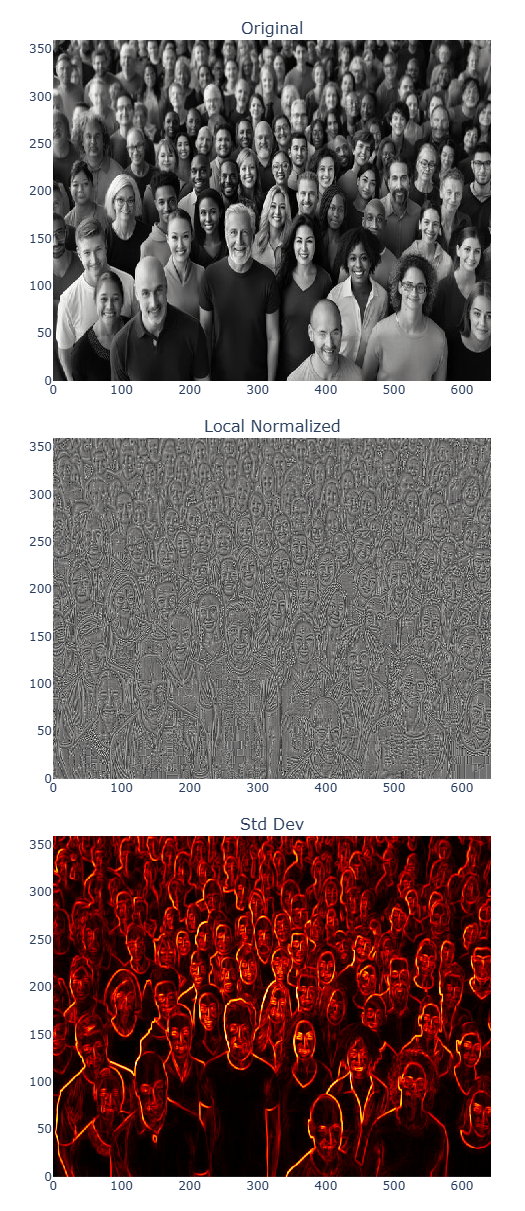
\includegraphics[width=\linewidth]{images/filter_crowd.png}
        \caption{Imagen de multitud con sus correspondientes filtros. De arriba abajo: original, normalizada localmente y desviación estándar.}
        \label{fig:filter_crowd}
    \end{subfigure}
    \hfill
    \begin{subfigure}[t]{0.55\textwidth}
        \centering
        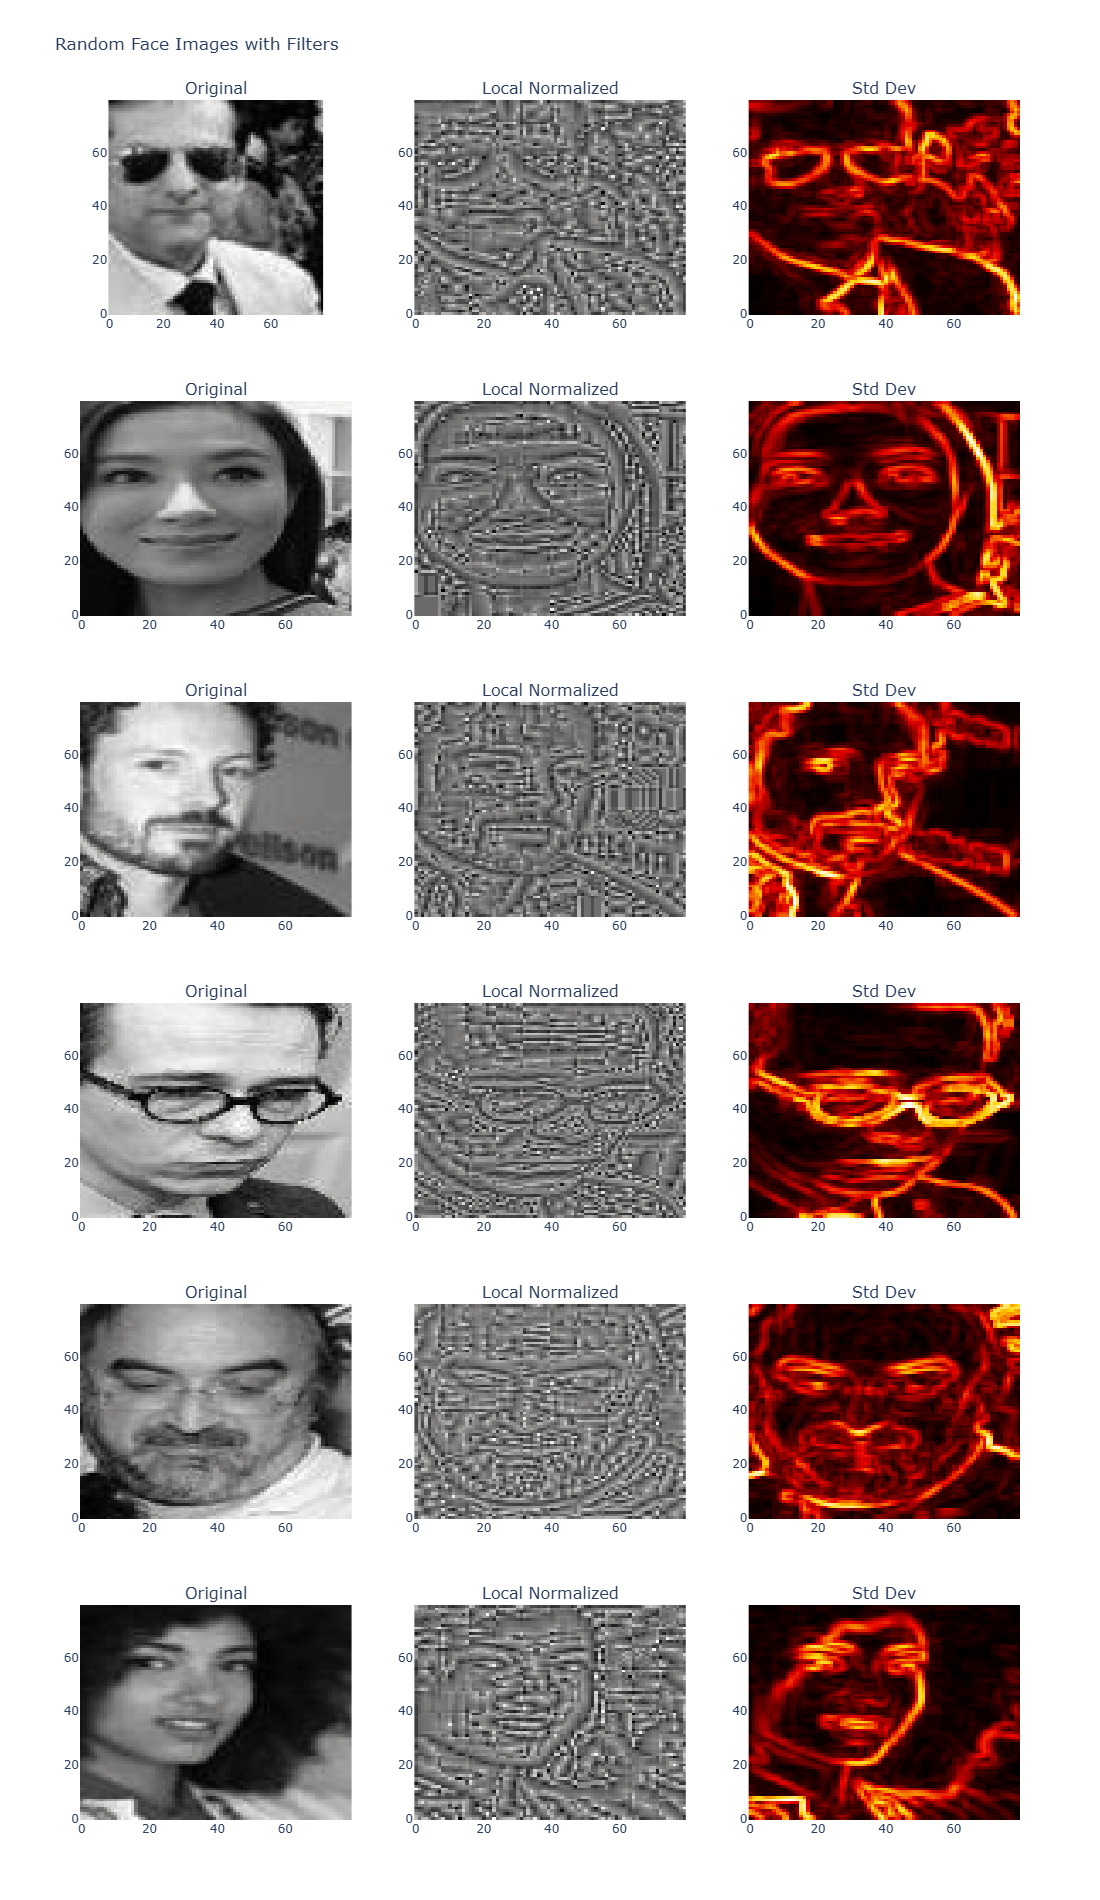
\includegraphics[width=\linewidth]{images/filter_onlyfaces.png}
        \caption{Malla de caras individuales mostrando el efecto de los filtros. Cada fila presenta, de izquierda a derecha: original, normalizada localmente y desviación estándar.}
        \label{fig:filter_faces}
    \end{subfigure}
    \caption{Resultados de la normalización local y el cálculo de desviación estándar sobre imágenes de multitud (izquierda) y caras individuales (derecha).}
    \label{fig:filtros}
\end{figure}



%%%%%%%%%%%%%%%%%%%%%%%%%%%%%%%%%%%%%%%%%%%%%%%%%%%%%%%%%%%%%%%%%%%%%%%%%%%%%
%                        Curva ROC                                       %
%%%%%%%%%%%%%%%%%%%%%%%%%%%%%%%%%%%%%%%%%%%%%%%%%%%%%%%%%%%%%%%%%%%%%%%%%%%%%
\chapter{Curva ROC}

La curva ROC es una herramienta para evaluar un sistema de clasificación, permite visualizar el compromiso entre TPR, \textit{True Positive Rate} y la FPR, \textit{False Positive Rate} al variar el umbral de decisión del clasificador. 

En este trabajo se ha implementado un \textit{notebook} que, dado un conjunto de puntuaciones de clientes e impostores, calcula estos ratios de forma exhaustiva para todos los umbrales posibles.

Se han utilizado dos conjuntos de datos, denominados A y B, cada uno con 2\,990 muestras (clientes e impostores mezclados). Las puntuaciones representan la confianza del sistema de que una muestra pertenece a un cliente legítimo. Para un umbral dado $\theta$, se definen:

\begin{itemize}
    \item \textbf{Falsos Positivos (FP)}: impostores clasificados erróneamente como clientes ($\text{score} > \theta$).
    \item \textbf{Falsos Negativos (FN)}: clientes rechazados erróneamente ($\text{score} \leq \theta$).
\end{itemize}

A partir de estos valores se computan las tasas $\text{FPR}$ y $\text{FNR}$ para cada umbral, permitiendo trazar la curva ROC ($\text{TPR} = 1 - \text{FNR}$ frente a FPR). Además, se calcula el área bajo la curva (AUC) mediante integración numérica por el método del trapecio (que se calcula en tiempo lineal, en lugar de cuadrático comparando todos los clientes con los impostores como hacemos en clase con pocos datos), obteniendo una métrica global de la capacidad discriminativa del sistema.

\begin{table}[H]
    \centering
    \begin{tabular}{lccl}
        \toprule
        \textbf{Métrica} & \textbf{Dataset A} & \textbf{Dataset B} & \textbf{Umbrales ($\theta_A$ / $\theta_B$)} \\
        \midrule
        AUC & 0,8831 & 0,8830 & — \\
        D prime & 0.7597 & 0.8732 & — \\
        \midrule
        FN = FP & 20,14\% & 20,07\% & $0{,}0503$ | $0{,}0444$ \\
        \rule{0pt}{3ex}
        FP para FN = 1\% & 80,13\% & 68,00\% & $0{,}0071$ | $0{,}0000$ \\
        FP para FN = 5\% & 57,56\% & 53,65\% & $0{,}0202$ | $0{,}0048$ \\
        FP para FN = 20\% & 20,45\% & 20,13\% & $0{,}0500$ | $0{,}0443$ \\
        \rule{0pt}{3ex}
        FN para FP = 1\% & 62,73\% & 64,55\% & $0{,}1474$ | $0{,}2999$ \\
        FN para FP = 5\% & 39,58\% & 44,55\% & $0{,}0826$ | $0{,}1444$ \\
        FN para FP = 20\% & 20,14\% & 20,42\% & $0{,}0504$ | $0{,}0450$ \\

        \bottomrule
    \end{tabular}
    \caption{Resultados principales del análisis ROC para los datasets A y B.}
    \label{tab:roc_results}
\end{table}

Los resultados, resumidos en la Tabla~\ref{tab:roc_results}, muestran que ambos datasets presentan un comportamiento muy similar, con un AUC cercano a 0,88, lo que indica una buena capacidad de discriminación del sistema. No obstante, el punto de igual error (donde $\text{FN} \approx \text{FP}$) se sitúa en torno al 20\%, lo cual sugiere que, para aplicaciones biométricas exigentes, sería necesario ajustar el umbral en función de si se prioriza minimizar los falsos positivos o los falsos negativos.

Por ejemplo, si se fija un umbral de $\theta = 0{,}10$, el dataset A presenta una tasa de FP del 2,63\% y una tasa de FN del 48,04\%, mientras que el dataset B arroja valores de 8,53\% y 34,62\%, respectivamente. Estas diferencias evidencian que la distribución de puntuaciones varía entre conjuntos de datos, por lo que la elección del umbral debe adaptarse al escenario de aplicación concreto.

Para obtener una tasa de FN en torno al 1\% (apenas rechazar clientes) es necesario reducir drásticamente el umbral. En el dataset A se requiere un umbral de $0{,}0071$, mientras que en el dataset B ni siquiera existe un umbral positivo que consiga ese FN, por lo que el valor más cercano es $\theta = 0{,}0000$, equivalente a aceptar toda puntuación mayor que cero. Ni siquiera con $\theta = 0$ se alcanza un FP del 100\%, ya que aproximadamente un 31\% de los impostores tiene puntuación exactamente cero y, por tanto, son correctamente rechazados.

\begin{figure}[H]
    \centering
    
\includegraphics[width=0.9\linewidth]{images/curva_roc.png}
    \caption{Curva ROC para los datasets A y B.}
    \label{fig:roc_curve}
\end{figure}

Ambos datasets muestran curvas prácticamente solapadas, lo que confirma que el sistema de puntuación se comporta de forma similar en ambos conjuntos. El AUC cercano a 0,88 indica una capacidad de discriminación aceptable, aunque la zona de bajo FP revela una caída pronunciada de la TPR, reflejando la dificultad de mantener una alta tasa de acierto cuando se exige una tasa de falsos positivos muy reducida.
%%%%%%%%%%%%%%%%%%%%%%%%%%%%%%%%%%%%%%%%%%%%%%%%%%%%%%%%%%%%%%%%%%%%%%%%%%%%%
%                        VIOLA JONES                                       %
%%%%%%%%%%%%%%%%%%%%%%%%%%%%%%%%%%%%%%%%%%%%%%%%%%%%%%%%%%%%%%%%%%%%%%%%%%%%%
\chapter{Viola Jones}
La implementación sigue fielmente el \textit{paper} original de Viola y Jones, con varias optimizaciones adicionales. Las fases principales son: (1) obtención de datos, (2) listado de características Haar, (3) selección de características con AdaBoost, (4) \textit{hard negative mining} y (5) clasificación en cascada.

\section{Obtención de datos}

\subsection{Dataset de NO caras}
Las muestras negativas se extraen del conjunto \texttt{open-images-v7} mediante \texttt{fiftyone}. Para garantizar la ausencia de caras, se filtran imágenes usando etiquetas que casi siempre implican ausencia de personas (\textit{Ant}, \textit{Apple}, \textit{Banana}...) y se excluyen etiquetas que puedan incluirlas (\textit{Human face}, \textit{Human arm}...). Las imágenes restantes se filtran con el detector OpenCV para eliminar cualquier cara residual. El resultado son más de 128\,000 imágenes sin caras.

El conjunto se divide en 90\% entrenamiento y 10\% test. Del 10\% de test se generan 2,5\,M de \textit{crops} estáticos para monitorizar la tasa de FP a lo largo del entrenamiento.

\begin{figure}[H]
  \centering
  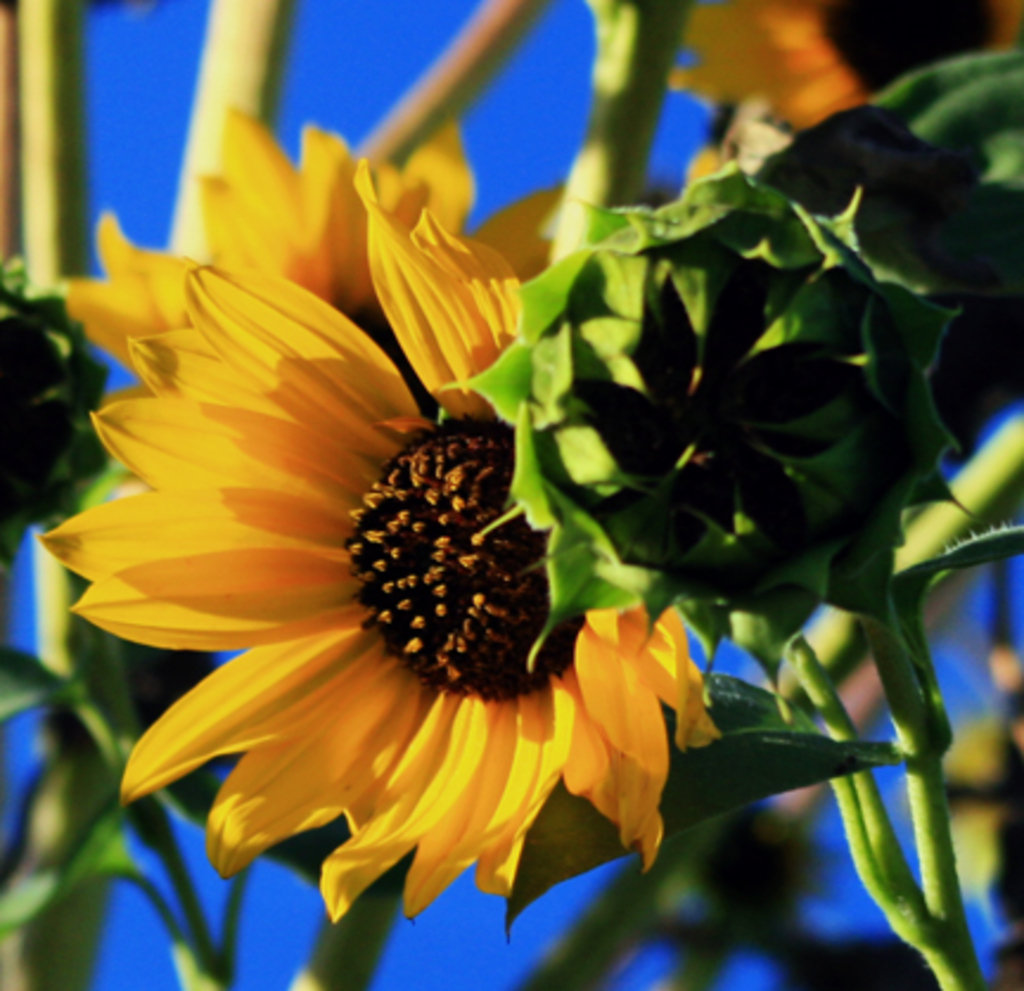
\includegraphics[width=0.3\linewidth]{images/no_caras/nocaras_1.jpg}
  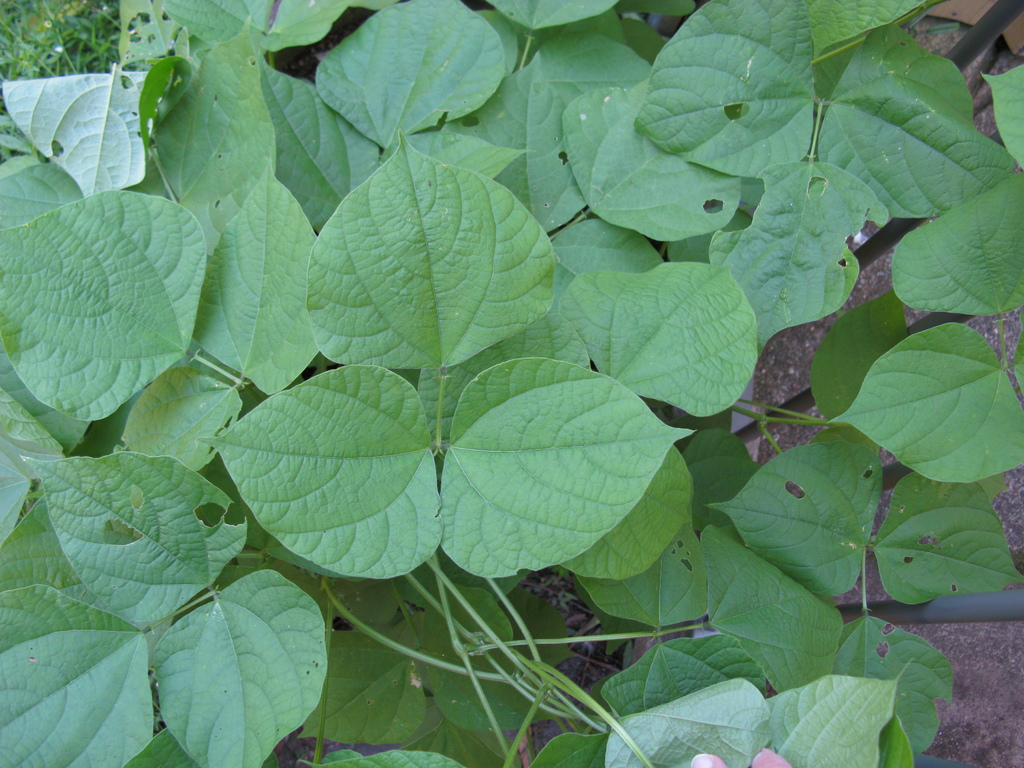
\includegraphics[width=0.3\linewidth]{images/no_caras/nocaras_2.jpg}
  \vspace{0.5cm}

  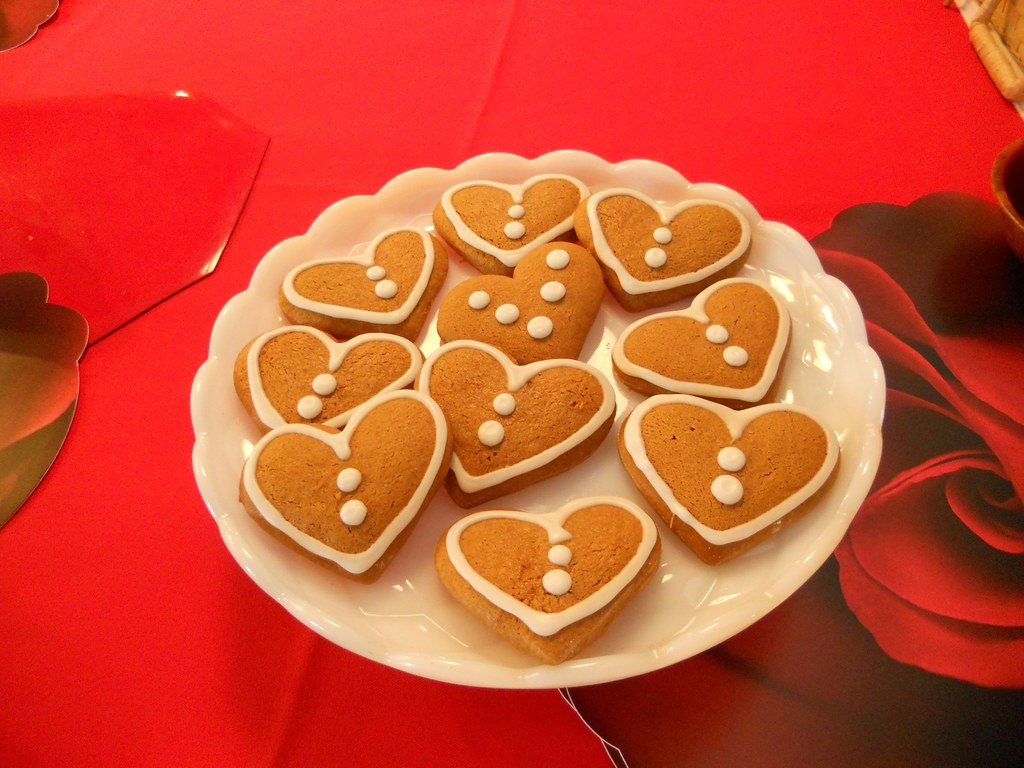
\includegraphics[width=0.3\linewidth]{images/no_caras/nocaras_3.jpg}
  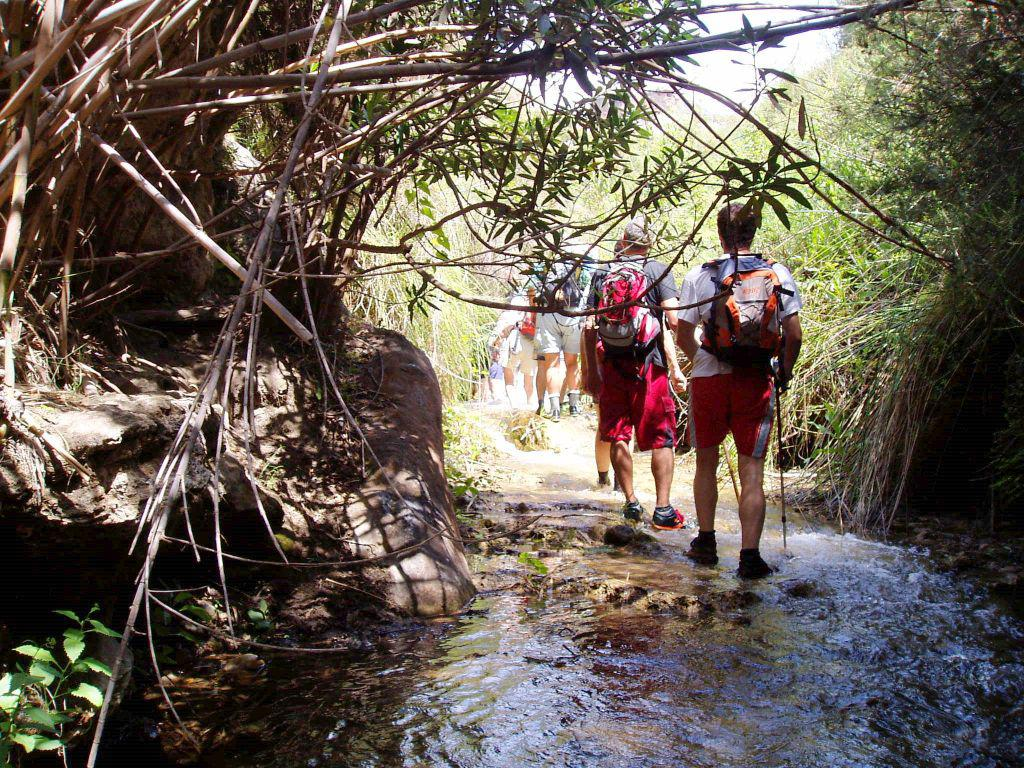
\includegraphics[width=0.3\linewidth]{images/no_caras/nocaras_4.jpg}
  \caption{Ejemplos de imágenes sin caras extraídas de Open Images V7.}
  \label{fig:no_caras}
\end{figure}

\subsection{Dataset de caras}
Las caras del \textit{dataset} original no están centradas ni alineadas (Figura~\ref{fig:caras_avg}, imagen izquierda). Se procesan con el detector de OpenCV, conservando solo los \textit{crops} con confianza superior a 8 (umbral normal: 5), lo que garantiza centrado en ojos y nariz. De 75\,k imágenes se obtienen 26\,k caras de 24$\times$24 px; con su versión espejo, más de 52\,k. Se reserva el 10\% para test.

\begin{figure}[H]
  \centering
  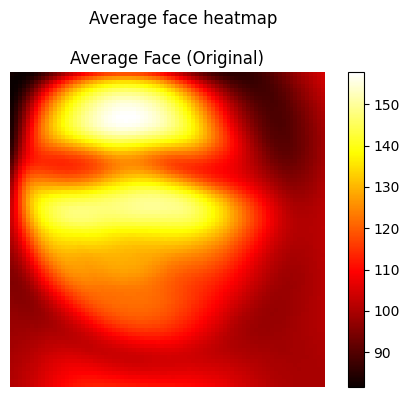
\includegraphics[width=0.275\linewidth]{images/caras/original_avg.png}
  \hspace{2.5cm}
  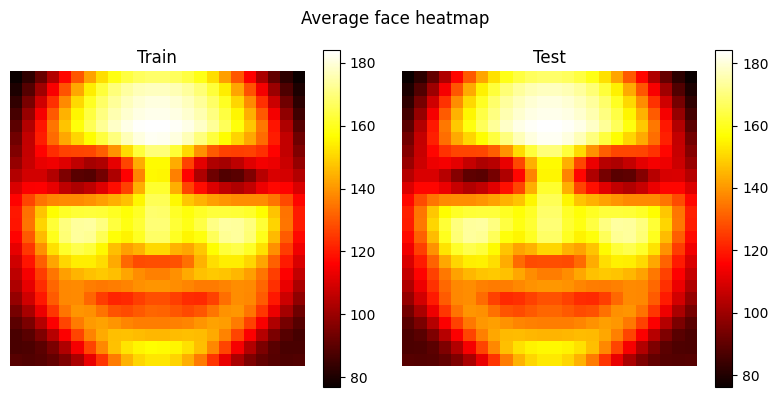
\includegraphics[width=0.50\linewidth]{images/caras/processed_avg.png}
  \caption{Cara media antes (izquierda, borrosa) y después (derecha) de procesar el dataset: los \textit{crops} centrados producen una cara nítida.}
  \label{fig:caras_avg}
\end{figure}

\section{Características Haar y AdaBoost}

\subsection{Listado de características}
Se recorren iterativamente todas las posiciones y tamaños de los filtros Haar sobre \textit{crops} de 24$\times$24 px. Los filtros invertidos se omiten porque AdaBoost determina el signo del peso asociado. Todos los valores se calculan mediante \textbf{imagen integral}.

Para reducir el espacio de características de 170\,k a ~81\,k, se limita el tamaño mínimo de cada filtro: horizontales 6$\times$4, verticales 4$\times$6, 3 horizontales 9$\times$4, 3 verticales 4$\times$9, diagonales 6$\times$6. Se añade además un filtro tipo marco (cuadrado con cuadrado concéntrico interior, mínimo 6$\times$6), sumando ~2\,k características más.

\begin{figure}[H]
    \centering
    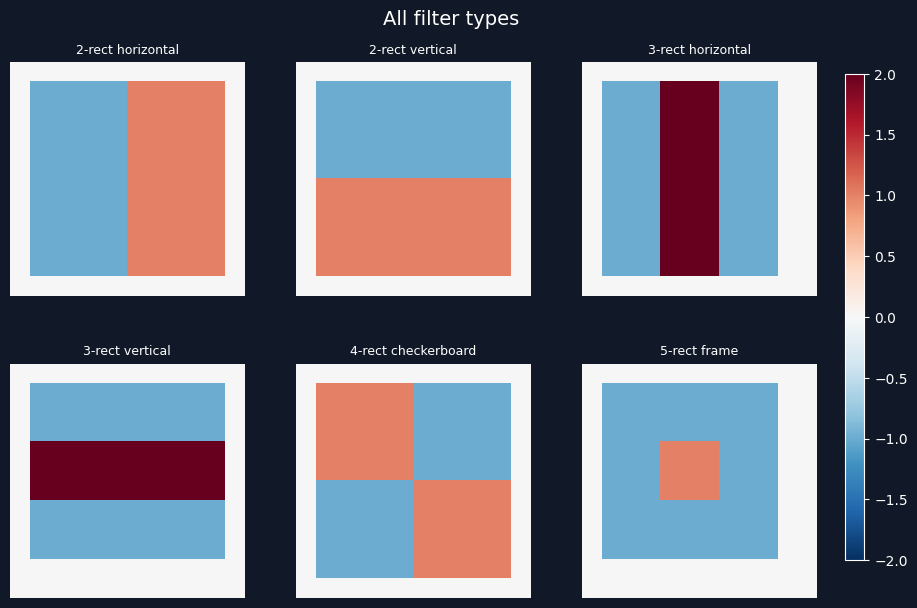
\includegraphics[width=0.5\linewidth]{images/filters/base-filters.png}
    \caption{Tipos de filtros Haar utilizados, incluido el filtro cuadrado concéntrico propuesto.}
    \label{fig:base-filters}
\end{figure}

\subsection{Selección con AdaBoost}
Se emplea una implementación personalizada de AdaBoost (con asistencia de Claude) con interfaz compatible con \texttt{scikit-learn}, especializada en \textit{stumps} y con búsqueda paralela del mejor \textit{split} por característica. Esta versión es significativamente más rápida que la estándar dado el volumen de características y muestras.

Tras cada \textit{stump}, se ajusta el umbral de etapa para garantizar TPR $\geq 0{,}999$ (o $\geq 0{,}99$ según configuración). Si el FP resultante alcanza el objetivo del 50\%, la etapa concluye; de lo contrario, se continúa hasta un máximo de 500 \textit{stumps}.
La elección de la TPR mínima tiene un efecto acumulativo importante: tras 30 etapas, una TPR de $0{,}99$ por etapa resulta en $0{,}99^{30} = 0{,}74$ de caras conservadas globalmente, frente a $0{,}999^{30} = 0{,}97$ con la configuración más estricta. Esto crea un compromiso directo entre la exigencia por etapa y la tasa de detección final.

Se experimenta también con una \textbf{tasa de FP progresiva}: etapas 1--2 con objetivo 15\%, etapas 3--5 con 25\%, etapas 6--10 con 40\%, y etapas 11+ con 50\%. El objetivo es que las primeras etapas, donde el \textit{hard mining} es menos exigente, eliminen más negativos aunque requieran más \textit{stumps}.

\section{Hard Mining y Clasificador en Cascada}

\subsection{Hard negative mining}
Para cada etapa, las muestras negativas se obtienen pasando imágenes de \texttt{open-images-v7} por la cascada acumulada: los \textit{crops} que superan todas las etapas previas son los falsos positivos más difíciles y conforman el conjunto negativo de entrenamiento. Este paso es esencial: no sirve precomputar un gran pool estático de negativos, ya que en pocas etapas el clasificador aprende a descartarlos y se queda sin muestras negativas útiles. Con \textit{hard mining} dinámico, cada etapa siempre se enfrenta a los casos más difíciles del momento.

\textbf{Preservación de FP heredados}: Los FP heredados de etapas anteriores se preservan y concatenan con los nuevos para evitar el olvido de patrones ya aprendidos. 

\textbf{Diversidad}: Para asegurar diversidad, se limita la extracción a un máximo del 10\% del total de \textit{crops} por imagen. Se pueden extraer menos si la imagen no tiene suficientes \textit{crops} que superen las etapas previas, pero no más para evitar sobre-representar ciertas imágenes.

\subsection{Clasificador en cascada}
El script \texttt{generate\_all\_stages} encadena las etapas, monitorizando la tasa global de FP sobre los 2,5\,M de \textit{crops} de test tras cada nueva etapa. El entrenamiento se detiene cuando se descarta la totalidad de los \textit{crops} de test o se alcanza el número máximo de etapas. El estado completo se guarda en \textit{checkpoint} tras cada etapa para permitir reanudar el entrenamiento si se interrumpe.

\section{Inferencia}
La versión de producción del clasificador (\texttt{app/src/model/cascade\_classifier.py}) está vectorizada y paralelizada con \texttt{numba} (\texttt{@njit(parallel=True)}), logrando evaluación en tiempo real. Para detectar caras a múltiples escalas se implementa una \textbf{pirámide de escalas} (factor de submuestreo 0,8 por defecto). Opcionalmente, se puede reducir la imagen de entrada a la mitad antes de iniciar la pirámide (\texttt{halve\_size\_factor}), lo que acelera significativamente la inferencia a costa de no detectar caras por debajo de un tamaño mínimo de \textit{crop}. 

\textbf{NMS}: Las detecciones solapadas se consolidan con \texttt{cv2.groupRectangles} (NMS, $\varepsilon=0{,}2$).

\textbf{Serialización}: El modelo se serializa con xml compatible con OpenCV para facilitar la comparación y uso de etapas preentrenadas.


%%%%%%%%%%%%%%%%%%%%%%%%%%%%%%%%%%%%%%%%%%%%%%%%%%%%%%%%%%%%%%%%%%%%%%%%%%%%%
%                        CONCLUSIONES Y RESULTADOS                         %
%%%%%%%%%%%%%%%%%%%%%%%%%%%%%%%%%%%%%%%%%%%%%%%%%%%%%%%%%%%%%%%%%%%%%%%%%%%%%
\chapter{Conclusiones y Resultados (Detector)}


Se realizan cinco experimentos variando dos parámetros: TPR mínima por etapa (0{,}999 / 0{,}99) y uso o no de tasa de FP progresiva. Los cuatro primeros usan 15\,000 muestras positivas y 15\,000 negativas por etapa; el quinto (\texttt{pfp\_999\_all\_data}) usa todas las muestras disponibles, entrenado en el clúster Tensor. Se muestra su progreso a lo largo de las etápas y resultados finales en test (FP = 0\% en todos los casos).

% \begin{figure}[H]
%     \centering
%     
\includegraphics[width=0.85\linewidth]{images/models/FP-TP-Progresion.png}
%     \caption{Progresión de FP y TPR a lo largo de las etapas para cada configuración.}
%     \label{fig:fp_tp_progression}
% \end{figure}



\begin{figure}[H]
\centering
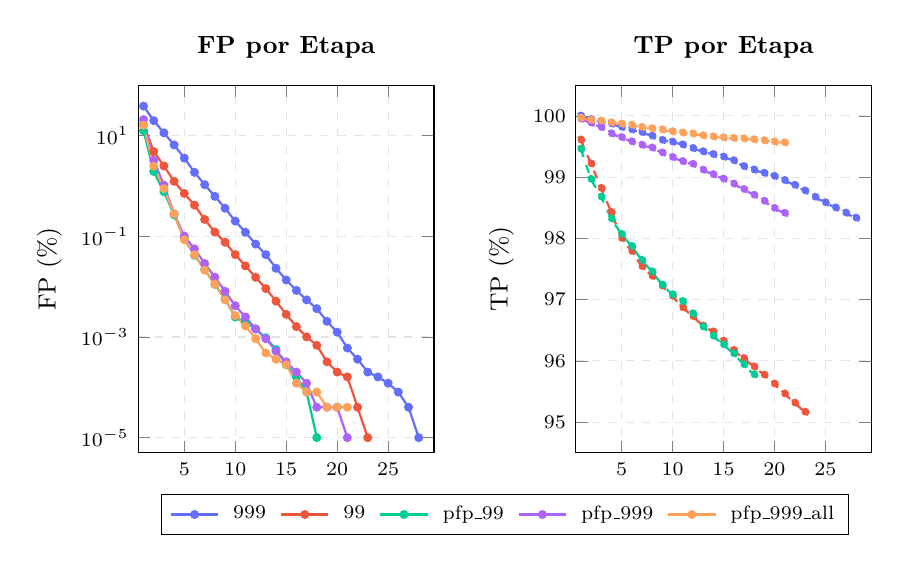
\begin{tikzpicture}
\definecolor{col999}{RGB}{99,110,250}
\definecolor{col99}{RGB}{239,85,59}
\definecolor{colpfp99}{RGB}{0,204,150}
\definecolor{colpfp999}{RGB}{171,99,250}
\definecolor{colpfp999all}{RGB}{255,161,90}

\begin{groupplot}[
    group style={group size=2 by 1, horizontal sep=1.8cm},
    width=0.44\textwidth,
    height=6.25cm,
    xlabel={Etapa},
    xtick={0,5,10,15,20,25},
    tick label style={font=\scriptsize},
    label style={font=\small},
    title style={font=\small\bfseries},
    grid=major,
    grid style={dashed, gray!20},
]

%% ── LEFT: FPR log scale ───────────────────────────────────────────
\nextgroupplot[
    title={FP por Etapa},
    ylabel={FP (\%)},
    ymode=log,
    ymin=5e-6, ymax=100,
    xmin=0.5, xmax=29.5,
    legend to name=pgflegend,
    legend style={legend columns=5, font=\scriptsize, column sep=3pt},
]

\addplot[color=col999,       solid, mark=*, mark size=1.2pt, line width=0.8pt] coordinates {
    (1,38.44)(2,19.78)(3,11.32)(4,6.51)(5,3.57)(6,1.86)(7,1.06)(8,0.62)
    (9,0.36)(10,0.20)(11,0.12)(12,0.07)(13,0.04319)(14,0.02312)(15,0.01353)
    (16,0.008390)(17,0.005459)(18,0.003653)(19,0.002047)(20,0.001244)
    (21,0.0006021)(22,0.0003613)(23,0.0002007)(24,0.0001606)(25,0.0001204)
    (26,0.00008028)(27,0.00004014)(28,0.00001)
}; \addlegendentry{999}

\addplot[color=col99,        solid, mark=*, mark size=1.2pt, line width=0.8pt] coordinates {
    (1,16.60)(2,4.821)(3,2.488)(4,1.233)(5,0.7081)(6,0.4148)(7,0.2156)
    (8,0.1211)(9,0.07595)(10,0.04327)(11,0.02573)(12,0.01529)(13,0.009152)
    (14,0.005138)(15,0.002810)(16,0.001606)(17,0.001004)(18,0.0006824)
    (19,0.0003211)(20,0.0002007)(21,0.0001606)(22,0.00004014)(23,0.00001)
}; \addlegendentry{99}

\addplot[color=colpfp99,     solid, mark=*, mark size=1.2pt, line width=0.8pt] coordinates {
    (1,12.50)(2,1.937)(3,0.7650)(4,0.2663)(5,0.08871)(6,0.04187)(7,0.02208)
    (8,0.01112)(9,0.005620)(10,0.002489)(11,0.001967)(12,0.001445)
    (13,0.0009634)(14,0.0005620)(15,0.0002810)(16,0.0001606)(17,0.00008028)
    (18,0.00001)
}; \addlegendentry{pfp\_99}

\addplot[color=colpfp999,    solid, mark=*, mark size=1.2pt, line width=0.8pt] coordinates {
    (1,20.74)(2,3.223)(3,1.035)(4,0.2783)(5,0.1009)(6,0.05636)(7,0.02882)
    (8,0.01541)(9,0.008069)(10,0.004175)(11,0.002489)(12,0.001445)
    (13,0.0009233)(14,0.0005219)(15,0.0003211)(16,0.0002007)(17,0.0001204)
    (18,0.00004014)(19,0.00004014)(20,0.00004014)(21,0.00001)
}; \addlegendentry{pfp\_999}

\addplot[color=colpfp999all, solid, mark=*, mark size=1.2pt, line width=0.8pt] coordinates {
    (1,16.01)(2,2.467)(3,0.8799)(4,0.2789)(5,0.08482)(6,0.04283)(7,0.02115)
    (8,0.01124)(9,0.005459)(10,0.002649)(11,0.001646)(12,0.0009233)
    (13,0.0004817)(14,0.0003613)(15,0.0002810)(16,0.0001204)(17,0.00008028)
    (18,0.00008028)(19,0.00004014)(20,0.00004014)(21,0.00004014)
}; \addlegendentry{pfp\_999\_all}

%% ── RIGHT: TPR linear scale ───────────────────────────────────────
\nextgroupplot[
    title={TP por Etapa},
    ylabel={TP (\%)},
    ymin=94.5, ymax=100.5,
    xmin=0.5, xmax=29.5,
    ytick={95,96,97,98,99,100},
]

\addplot[color=col999,       dashed, mark=*, mark size=1.2pt, line width=0.8pt] coordinates {
    (1,99.996)(2,99.939)(3,99.895)(4,99.867)(5,99.813)(6,99.772)(7,99.729)
    (8,99.668)(9,99.600)(10,99.572)(11,99.526)(12,99.467)(13,99.414)
    (14,99.368)(15,99.327)(16,99.268)(17,99.172)(18,99.116)(19,99.063)
    (20,99.012)(21,98.944)(22,98.866)(23,98.774)(24,98.671)(25,98.581)
    (26,98.497)(27,98.413)(28,98.331)
};

\addplot[color=col99,        dashed, mark=*, mark size=1.2pt, line width=0.8pt] coordinates {
    (1,99.606)(2,99.217)(3,98.815)(4,98.423)(5,97.999)(6,97.786)(7,97.540)
    (8,97.380)(9,97.220)(10,97.054)(11,96.867)(12,96.724)(13,96.570)
    (14,96.473)(15,96.322)(16,96.170)(17,96.037)(18,95.903)(19,95.768)
    (20,95.622)(21,95.461)(22,95.311)(23,95.163)
};

\addplot[color=colpfp99,     dashed, mark=*, mark size=1.2pt, line width=0.8pt] coordinates {
    (1,99.455)(2,98.963)(3,98.673)(4,98.317)(5,98.064)(6,97.868)(7,97.640)
    (8,97.455)(9,97.238)(10,97.080)(11,96.970)(12,96.769)(13,96.553)
    (14,96.402)(15,96.264)(16,96.117)(17,95.938)(18,95.774)
};

\addplot[color=colpfp999,    dashed, mark=*, mark size=1.2pt, line width=0.8pt] coordinates {
    (1,99.947)(2,99.881)(3,99.809)(4,99.707)(5,99.645)(6,99.576)(7,99.520)
    (8,99.475)(9,99.395)(10,99.321)(11,99.254)(12,99.209)(13,99.114)
    (14,99.040)(15,98.967)(16,98.887)(17,98.798)(18,98.704)(19,98.606)
    (20,98.489)(21,98.409)
};

\addplot[color=colpfp999all, dashed, mark=*, mark size=1.2pt, line width=0.8pt] coordinates {
    (1,99.963)(2,99.928)(3,99.916)(4,99.887)(5,99.865)(6,99.846)(7,99.811)
    (8,99.791)(9,99.770)(10,99.742)(11,99.721)(12,99.705)(13,99.674)
    (14,99.656)(15,99.641)(16,99.633)(17,99.625)(18,99.610)(19,99.594)
    (20,99.574)(21,99.559)
};

\end{groupplot}

%% Shared legend centered below both plots
\node[below=0.4cm] at ($(group c1r1.south)!0.5!(group c2r1.south)$)
    {\pgfplotslegendfromname{pgflegend}};

\end{tikzpicture}
\caption{Progresión de la tasa de FP (escala logarítmica, línea sólida) y TPR (línea discontinua) a lo largo de las etapas del clasificador en cascada para cada configuración.}
\label{fig:fp_tp_progression}
\end{figure}






\begin{table}[H]
    \centering
    \small % Reduces font size slightly for a tighter fit
    \begin{tabular}{llcc}
        \toprule
        \textbf{Modelo} & \textbf{Descripción} & \textbf{Etapas} & \textbf{TPR final} \\
        \midrule
        \texttt{balanced\_999} & TPR $\geq 0{,}999$, FP fijo & 28 & 0,9833 \\
        \texttt{balanced\_99}  & TPR $\geq 0{,}99$, FP fijo  & 23 & 0,9516 \\
        \texttt{pfp\_99}       & TPR $\geq 0{,}99$, FP progresivo  & 18 & 0,9577 \\
        \texttt{pfp\_999}      & TPR $\geq 0{,}999$, FP progresivo & 21 & 0,9841 \\
        \texttt{pfp\_999\_all}* & TPR $\geq 0{,}999$, FP progresivo & 21 & \textbf{0,9956} \\
        \bottomrule
    \end{tabular}
    \caption{Configuraciones y resultados. Todos los modelos alcanzan FP = 0\% en test. (*Con todos los datos).}
    \label{tab:model_configs}
\end{table}
% \subsection{Filtros Haar por etapa}

\begin{table}[H]
    \centering
    \resizebox{\textwidth}{!}{
    \begin{tabular}{l*{28}{r}|r}
        \toprule
        \textbf{Modelo} & \textbf{S0} & \textbf{S1} & \textbf{S2} & \textbf{S3} & \textbf{S4} & \textbf{S5} & \textbf{S6} & \textbf{S7} & \textbf{S8} & \textbf{S9} & \textbf{S10} & \textbf{S11} & \textbf{S12} & \textbf{S13} & \textbf{S14} & \textbf{S15} & \textbf{S16} & \textbf{S17} & \textbf{S18} & \textbf{S19} & \textbf{S20} & \textbf{S21} & \textbf{S22} & \textbf{S23} & \textbf{S24} & \textbf{S25} & \textbf{S26} & \textbf{S27} & \textbf{Total} \\
        \midrule
        \texttt{99}       & 2 & 5 & 5 & 8 & 6 & 12 & 15 & 23 & 26 & 36 & 37 & 40 & 54 & 62 & 67 & 77 & 90 & 93 & 123 & 125 & 141 & 157 & 178 & -- & -- & -- & -- & -- & \textbf{1382} \\
        \texttt{999}      & 4 & 6 & 8 & 11 & 15 & 24 & 30 & 38 & 44 & 56 & 70 & 76 & 93 & 112 & 128 & 141 & 157 & 187 & 202 & 222 & 256 & 284 & 330 & 346 & 367 & 419 & 475 & 500 & \textbf{4601} \\
        \texttt{pfp\_99}  & 4 & 10 & 13 & 22 & 39 & 36 & 47 & 56 & 68 & 87 & 84 & 91 & 98 & 112 & 133 & 137 & 159 & 178 & -- & -- & -- & -- & -- & -- & -- & -- & -- & -- & \textbf{1374} \\
        \texttt{pfp\_999} & 7 & 23 & 38 & 59 & 86 & 85 & 109 & 133 & 155 & 181 & 186 & 218 & 225 & 246 & 302 & 317 & 355 & 395 & 414 & 452 & 500 & -- & -- & -- & -- & -- & -- & -- & \textbf{4486} \\
        \texttt{pfp\_999\_all} & 11 & 34 & 52 & 85 & 136 & 153 & 188 & 250 & 302 & 371 & 370 & 443 & 500 & 500 & 500 & 500 & 500 & 500 & 500 & 500 & 500 & -- & -- & -- & -- & -- & -- & -- & \textbf{6895} \\
        \bottomrule
    \end{tabular}
    }
    \caption{Número de filtros Haar seleccionados por etapa en cada configuración.}
    \label{tab:haar_filters}
\end{table}

Los modelos con TPR $\geq 0{,}999$ requieren notablemente más filtros (\texttt{balanced\_999}: 4\,601 frente a 1\,382 de \texttt{balanced\_99}). En \texttt{pfp\_999\_all}, 9 de las 21 etapas alcanzan el máximo de 500 \textit{stumps} sin llegar al objetivo de FP, lo que indica que la mayor diversidad de datos requeriría un límite más alto de \textit{stumps} para una convergencia más rápida.

\subsection{Filtros de la primera etapa}

\begin{figure}[H]
    \centering
    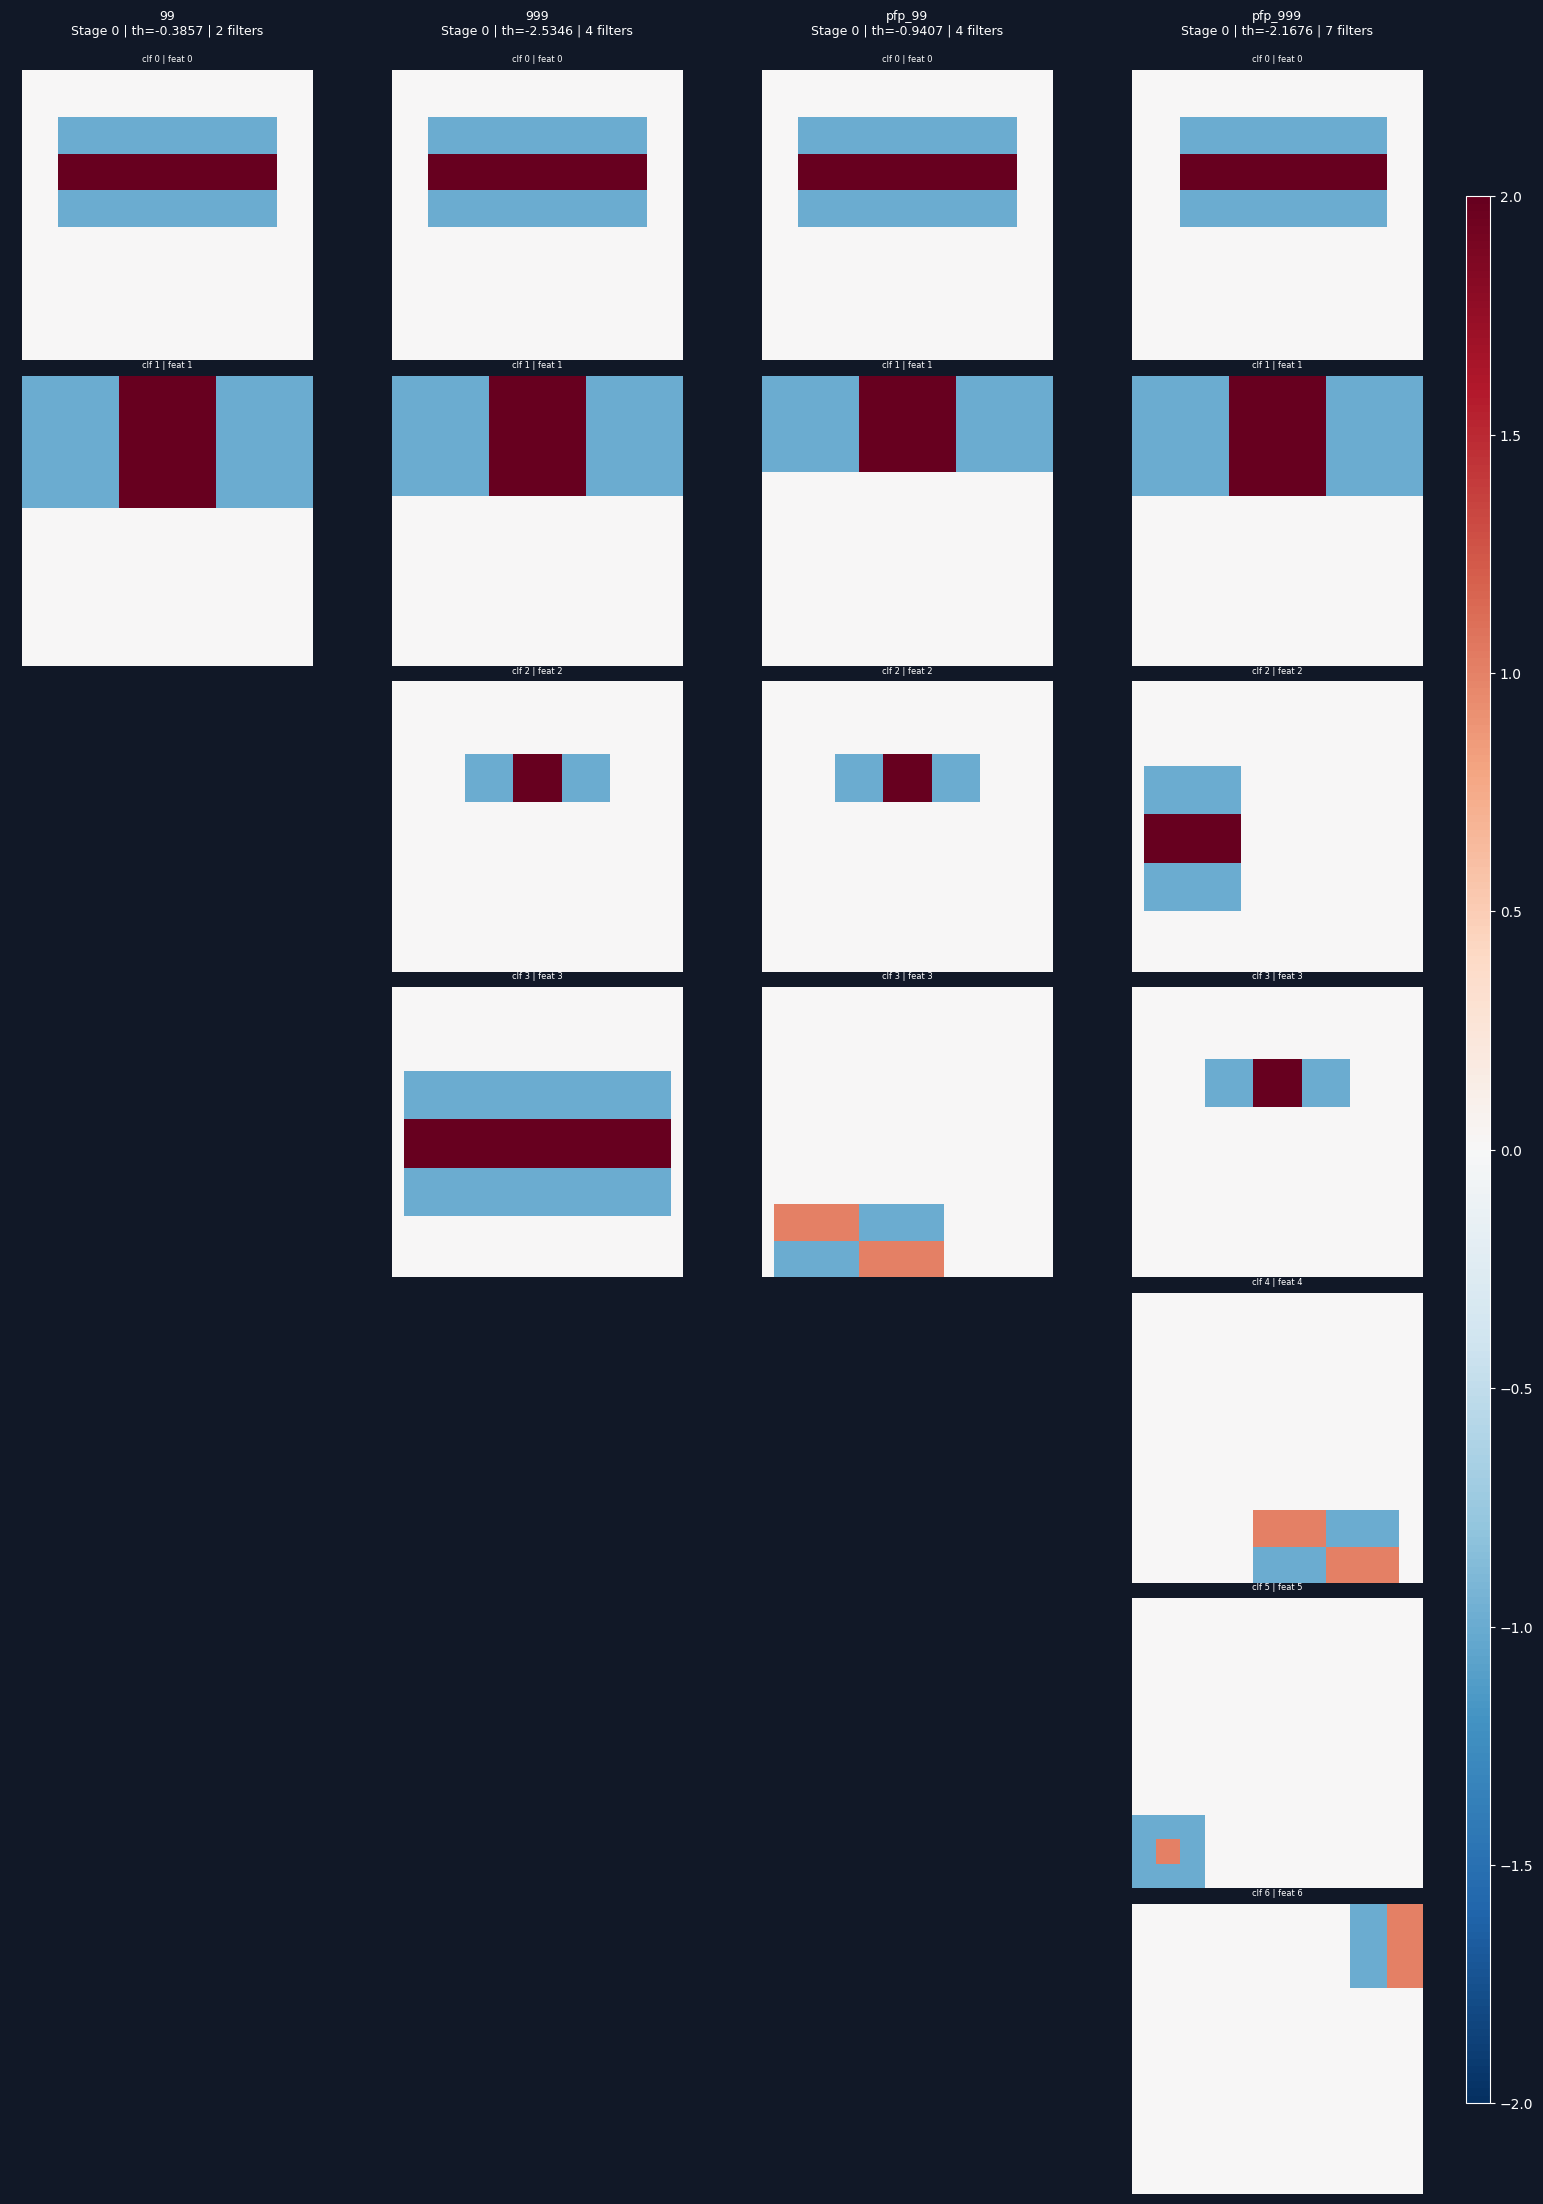
\includegraphics[width=0.8\linewidth]{images/models/first-Stage.png}
    \caption{Filtros Haar de la primera etapa para cada configuración (de izquierda a derecha: \texttt{nopfp\_99}, \texttt{nopfp\_999}, \texttt{pfp\_99}, \texttt{pfp\_999}, \texttt{pfp\_999\_all\_data}).}
    \label{fig:first_stage}
\end{figure}

Los primeros 2--3 filtros son prácticamente idénticos en todas las configuraciones (contraste ojos-frente, nariz-mejillas), confirmando que estas son las características faciales más discriminativas. El filtro cuadrado concéntrico propuesto apenas aparece en ninguna configuración, lo que indica que no aporta valor adicional sobre los filtros Haar clásicos.

\subsection{Inferencia en tiempo real}

\begin{table}[H]
    \centering
    \begin{tabular}{lcc}
        \toprule
        \textbf{Modelo} & \textbf{FPS} & \textbf{Observaciones} \\
        \midrule
        \texttt{balanced\_99}  & $\sim$\textbf{72,3} & Menor precisión \\
        \texttt{balanced\_999} & $\sim$60,5 & Detección robusta \\
        \texttt{pfp\_99}       & $\sim$69,0 & Menor precisión \\
        \texttt{pfp\_999}      & $\sim$59,3 & Detección robusta \\
        \texttt{pfp\_999\_all} & $\sim$53,1 & Detección robusta \\
        \bottomrule
    \end{tabular}
    \caption{Velocidad de inferencia en tiempo real para cada configuración.}
    \label{tab:inference_fps}
\end{table}

Todos los modelos superan ampliamente los 30 FPS. Los modelos TPR $\geq 0{,}99$ alcanzan $\sim$70 FPS frente a $\sim$60 FPS de los de 0{,}999, con \texttt{pfp\_999\_all} en $\sim$53 FPS. La tasa progresiva de FP no aporta ventaja en velocidad: aunque reduce el número de etapas, concentra más \textit{stumps} en cada una, resultando en un número total prácticamente idéntico. La diferencia real está en la calidad de detección: los modelos 0{,}99 presentan fallos frecuentes con gafas y rotaciones de cabeza que los de 0{,}999 manejan con mayor robustez.

\section{Conclusiones}

\begin{itemize}
    \item \textbf{TPR $\geq 0{,}999$ vs. $0{,}99$}: La TPR mínima por etapa es el factor determinante del rendimiento final. Los modelos 0{,}999 son superiores en robustez (seguimiento en rotación, invarianza a gafas) con una penalización moderada en velocidad ($\sim$10 FPS) que no compromete la operación en tiempo real. \texttt{pfp\_999\_all} alcanza la TPR final más alta (0,9956) a 53 FPS.

    \item \text{Progressive FPR}: Un resultado relevante es que la tasa progresiva de FP no aporta ventaja en velocidad. Aunque reduce el número de etapas, concentra más \textit{stumps} en cada una, y dado que las etapas anteriores procesan un mayor número de \textit{crops} (todavía no descartados por la cascada), el coste computacional total resulta prácticamente idéntico o ligeramente superior: \texttt{pfp\_99} a 69{,}0 FPS frente a \texttt{balanced\_99} a 72{,}3; \texttt{pfp\_999} a 59{,}3 frente a \texttt{balanced\_999} a 60{,}5. La mejora en TPR es igualmente marginal ($<$0{,}01).

    \item \textbf{Escalado con datos}: \texttt{pfp\_999\_all} es el modelo más lento y con más filtros (6\,895), con 9 etapas saturando el límite de 500 \textit{stumps}. Su TPR desciende más gradualmente, lo que indica que mayor diversidad de datos dificulta la convergencia pero produce un clasificador más robusto. Aumentar el límite de \textit{stumps} o el número de etapas podría mejorar aún más el resultado.

    \item \textbf{Filtros Haar}: Las características más discriminativas (contraste ojos-frente, nariz-mejillas) son consistentes en todas las configuraciones. El filtro cuadrado concéntrico propuesto no ha aportado valor adicional sobre los filtros clásicos.

    \item \textbf{Optimizaciones}: La paralelización del AdaBoost, la vectorización con \texttt{numba} y el \textit{hard negative mining} con preservación de FP han sido esenciales para hacer viable el entrenamiento (~45\,s/\textit{stump}) y alcanzar detección en tiempo real en todas las configuraciones.
\end{itemize}

%%%%%%%%%%%%%%%%%%%%%%%%%%%%%%%%%%%%%%%%%%%%%%%%%%%%%%%%%%%%%%%%%%%%%%%%%%%%%%%
%                                                                             %
%                                BIBLIOGRAFIA                                 %
%                                                                             %
%%%%%%%%%%%%%%%%%%%%%%%%%%%%%%%%%%%%%%%%%%%%%%%%%%%%%%%%%%%%%%%%%%%%%%%%%%%%%%%
\cleardoublepage
\printbibliography

%%%%%%%%%%%%%%%%%%%%%%%%%%%%%%%%%%%%%%%%%%%%%%%%%%%%%%%%%%%%%%%%%%%%%%%%%%%%%%%
%                                                                             %
%                                 APÉNDICES                                  %
%                                                                             %
%%%%%%%%%%%%%%%%%%%%%%%%%%%%%%%%%%%%%%%%%%%%%%%%%%%%%%%%%%%%%%%%%%%%%%%%%%%%%%%

\APPENDIX


%%%%%%%%%%%%%%%%%%%%%%%%%%%%%%%%%%%%%%%%%%%%%%%%%%%%%%%%%%%%%%%%%%%%%%%%%%%%%%
%                       EJEMPLOS DE CADA TIPO DE FACTURA                     %
%%%%%%%%%%%%%%%%%%%%%%%%%%%%%%%%%%%%%%%%%%%%%%%%%%%%%%%%%%%%%%%%%%%%%%%%%%%%%%

% \chapter{Apéndice correspondencia notebooks}
% \label{appendix:notebooks}
% ...

%%%%%%%%%%%%%%%%%%%%%%%%%%%%%%%%%%%%%%%%%%%%%%%%%%%%%%%%%%%%%%%%%%%%%%%%%%%%%%%
%                              FIN DEL DOCUMENTO                              %
%%%%%%%%%%%%%%%%%%%%%%%%%%%%%%%%%%%%%%%%%%%%%%%%%%%%%%%%%%%%%%%%%%%%%%%%%%%%%%%
\end{document}

